\documentclass[conference]{IEEEtran}
	\makeatletter
	\def\ps@headings{%
	\def\@oddhead{\mbox{}\scriptsize\rightmark \hfil \thepage}%
	\def\@evenhead{\scriptsize\thepage \hfil \leftmark\mbox{}}%
	\def\@oddfoot{}%
	\def\@evenfoot{}}
	\makeatother
	\pagestyle{headings}
	
	\hyphenation{op-tical net-works semi-conduc-tor}
	
	
	\usepackage{subfigure}
	\usepackage{soul}
	
	\usepackage{listings}
	\usepackage{algorithmic}
	\usepackage[ruled,vlined]{algorithm2e}
	
	\ifCLASSINFOpdf
	  \usepackage[pdftex]{graphicx}
	  % declare the path(s) where your graphic files are
	  % \graphicspath{{../pdf/}{../jpeg/}}
	  % and their extensions so you won't have to specify these with
	  % every instance of \includegraphics
	  % \DeclareGraphicsExtensions{.pdf,.jpeg,.png}
	\else
	  % or other class option (dvipsone, dvipdf, if not using dvips). graphicx
	  % will default to the driver specified in the system graphics.cfg if no
	  % driver is specified.
	  % \usepackage[dvips]{graphicx}
	  % declare the path(s) where your graphic files are
	  % \graphicspath{{../eps/}}
	  % and their extensions so you won't have to specify these with
	  % every instance of \includegraphics
	  % \DeclareGraphicsExtensions{.eps}
	\fi
	% graphicx was written by David Carlisle and Sebastian Rahtz. It is
	% required if you want graphics, photos, etc. graphicx.sty is already
	% installed on most LaTeX systems. The latest version and documentation can
	% be obtained at:
	% http://www.ctan.org/tex-archive/macros/latex/required/graphics/
	% Another good source of documentation is "Using Imported Graphics in
	% LaTeX2e" by Keith Reckdahl which can be found as epslatex.ps or
	% epslatex.pdf at: http://www.ctan.org/tex-archive/info/
	%
	% latex, and pdflatex in dvi mode, support graphics in encapsulated
	% postscript (.eps) format. pdflatex in pdf mode supports graphics
	% in .pdf, .jpeg, .png and .mps (metapost) formats. Users should ensure
	% that all non-photo figures use a vector format (.eps, .pdf, .mps) and
	% not a bitmapped formats (.jpeg, .png). IEEE frowns on bitmapped formats
	% which can result in "jaggedy"/blurry rendering of lines and letters as
	% well as large increases in file sizes.
	%
	% You can find documentation about the pdfTeX application at:
	% http://www.tug.org/applications/pdftex
	
\begin{document}
\title{Implementation and analysis of\\the main path planning techniques}

% Author names 
% note positions of commas and nonbreaking spaces ( ~ ) LaTeX will not break
% a structure at a ~ so this keeps an author's name from being broken across
% two lines.
% use \thanks{} to gain access to the first footnote area
% a separate \thanks must be used for each paragraph as LaTeX2e's \thanks
% was not built to handle multiple paragraphs
\author{
	Alessandro Zini, Filippo Morselli, Carlo Stomeo
	\\
	\IEEEauthorblockA{
		Dipartimento di Informatica - Scienza e Ingegneria, University of Bologna, Italy
		\\
		Emails: alessandro.zini3@studio.unibo.it, filippo.morselli@studio.unibo.it, carlo.stomeo@studio.unibo.it
	}
}

\maketitle

\begin{abstract}
	This report describes the final project for the Mobile Systems course. The work that has been done represents the first part of a larger project, which aims at implementing different mobility algorithms for a rover equipped with sensors in a real-world environment with obstacles.

	In this first phase a JavaScript application, \textbf{Path Planner} \cite{Path-Planner}, has been developed, which provides a generic `playground'-platform for positioning and moving objects in a bi-dimensional grid-based environment. Within such environment, the most popular path planning approaches studied in the Mobile Systems course have been implemented, tested and compared.

	The final product of this phase consists of an application that implements a user customizable environment in respect to size, obstacle positioning, as well as start and destination point. Using the software it is possible to obtain a path from start towards the destination, with the possibility of varying the path planning algorithm.

	The main purpose of this work is to put into practice the path planning algorithms seen during the lessons and study them up to the implementation details. Another goal is to have an easily customizable and extensible software to use as a starting point for the second part of the project, that is the actual mobility of an agent in the real world.
\end{abstract}

\section{Introduction}
\emph{Path planning} is the process of determining the path an agent has to follow in order to reach a given destination. It's a problem with lot of variants, depending on the characteristics of the environment in which the entity has to move and also depending on the capabilities and knowledge of the entity itself.

The context that has been assumed during the making of the project is a bi-dimensional environment partitioned in a grid map. Each cell of the grid can be free or occupied by an obstacle object. Two of the free cells are marked as starting point and destination. The problem consist in finding the best possible path to reach the destination cell from the start position.

It is assumed that the dimension of the moving agent are always smaller that the one of the unit cell, therefore the path is defined as a sequence of free adjacent cells that lead the agent to the goal. Diagonal movements are allowed, provided that the agent does not go through two diagonally adjacent obstacles. Also, the environment is assumed to be static, so there can't be any modification to the displacement of obstacles once the path computation starts.

In such environment, two different versions of the problem have been analyzed: the \emph{global} or \emph{offline path planning} in which there is a full \emph{a priori} knowledge of the map configuration, and the \emph{local} or \emph{online path planning} where the only inputs are the starting position and the destination position and the agent discovers the presence of obstacles only when they are within a certain range, so to simulate proximity sensors.

For both kind of problems, the most popular techniques are implemented in order to study their behavior in different environment configurations and to compare their performances.

The implemented techniques are the following:
\begin{itemize}
	\item Cellular/Grid Decomposition
	\item Visibility Graph
	\item Probabilistic Roadmap
	\item Potential Field
	\item Bug (version 1 and version 2)
	\item Tangent Bug
\end{itemize}

The paper is organized as follows. In Section 2 there is a brief survey of related works and similar applications. Section 3 describes the architecture of the web application and the module used to implement it. Section 4 describes the implementation details of each path planning method adopted. In Section 5 a performance evaluation for the various algorithms is presented. Last, Section 6 illustrates the conclusions.

\section{Related works}
The first step we took in our work has been to look for projects similar to our concept. We found two projects (\cite{l1-path-finder} and \cite{PathFinding.js}) from which we borrowed some ideas regarding the layout of the project.
Path Planning has been described and studied in depth in the state of the art. Warren et al. \cite{warren1989global} proposed to use potential fields for robotic manipulators and mobile robots in the presence of stationary obstacles. In \cite{sariff2006overview} Sariff et al. presented an overview and discusses the strength and weakness of many path planning algorithms including Visibility Graph and Potential Fields. In \cite{yoonprobabilistic} Yoon et al. discuss in details the Probabilistic Roadmap approach: Geraerts et al.\ in \cite{geraerts2004comparative} analyze and compare many variants of this approach.
Regarding the implementation of Bug approaches, \cite{tgBugSlides} has been discovered to be a very useful resource; in addition, various different variation of Bug algorithms, including Bug v1, Bug v2 and Tangent Bug, are described, tested and compared on different environments by James et al. in \cite{ng2007performance}.

\section{Architecture}
While investigating the architecture for the software, the idea of developing a standalone web page has appeared to emerge among other choices. The primary reason for this choice was portability, followed by the advantage of previous experience by the members of the team in term of web development, and the general ease of programming of user interfaces in the web environment.

In order to provide a smooth and, when possible, lightweight experience, the use of external libraries has been reduced to the minimum; also, the `playground'-grid has been maximized in space, being the real focus of the software. The user interface has been realized in HTML5 using Materialize CSS, a front-end framework based on Material Design. A floating menu has been introduced to let the user have the control over which planning algorithm to use, and to have some other handy functions available, like obstacle clearance, \dots

The grid and all its graphic functionalities have been realized in pure HTML5 using the \texttt{canvas} element. To ease the development, we wrote a small library which takes responsibility for handling all the functionalities related to drawing both the grid and its elements (squares, circles, lines, \dots).
Lastly, all the algorithms have been implemented in JavaScript, subdivided by their family of belonging. When required, an external library has been used to compute the Dijkstra shortest path algorithm over a graph.

\section{Implementation}

\subsection{Cellular/Grid Decomposition}
A decomposition algorithm, as the name suggests, works by decomposing a continuous environment into a discrete grid, which is then properly translated into a graph where a shortest path algorithm (\emph{e.g.} Dijkstra) is applied. Such algorithms belong to the family of offline algorithms.
In this work, both Cellular and Grid Decomposition approaches have been grouped into a single approach, since the initial assumptions of the environment caused the two to be equivalent. A brief explanation is given below.

A \emph{Cellular Decomposition} algorithm goes through the following steps:
\begin{itemize}
	\item subdivide the free space F into connected regions (cells);
	\item determine which cells are adjacent and construct an adjacency graph, where vertices corresponds to cells and edges join cells that have a common boundary;
	\item search for a path in the adjacency graph between the cells corresponding to start and end points;
	\item from the path resulted from the previous step, compute a path connecting certain points of the cells such as their midpoints (centroids).
\end{itemize}

While such approach is very simplistic, it is not usable for 8-directional motion planning, since it requires extra movements other than the canonical N-NE-E-SE-S-SW-W-NW (Fig. \ref{fig:cellDecompositionAllowedDirections}).

\begin{figure}[]
	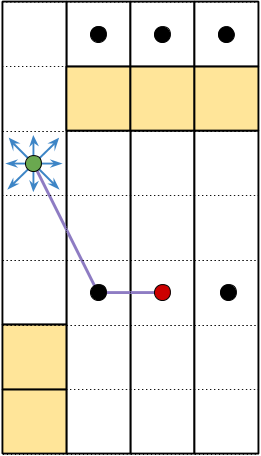
\includegraphics[width=4.5cm]{cell_decomposition_directions.png}
	\centering
	\caption{The blue arrows show the 8 (theoretical) allowed directions, while the purple line shows the path from source to destination obtained with the algorithm. The discrete grid environment assumed in this work is dotted in the background, while the resulting Cellular Decomposition cells are outlined in bold, with their centroid denoted by a black dot.}
	\label{fig:cellDecompositionAllowedDirections}
\end{figure}

To allow movements in 8 directions, the environment should be decomposed into squared tiles, which would cause the approach to behave identically as if the environment would have been decomposed into a grid (Fig. \ref{fig:cellDecompositionAllowedDirectionsGrid}), therefore causing it to degenerate into a Grid Decomposition method.

\begin{figure}[]
	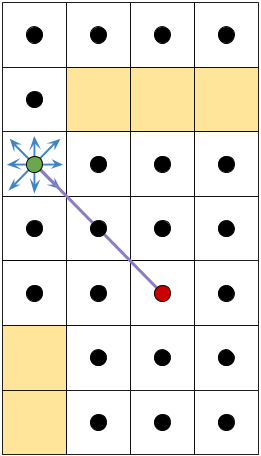
\includegraphics[width=4.5cm]{cell_decomposition_directions_grid.png}
	\centering
	\caption{A Cellular Decomposition approach degenerated into a Grid Decomposition method.}
	\label{fig:cellDecompositionAllowedDirectionsGrid}
\end{figure}

A simple \emph{Grid Decomposition} approach differs from the Cellular counterpart by how it subdivides the free space. It goes through the following steps:
\begin{itemize}
	\item decompose the space into a grid of cells of equal size;
	\item mark every cell either as \emph{free} or \emph{busy} depending on the presence of an obstacle inside.
	\item determine which free cells are adjacent and construct an adjacency graph, where vertices corresponds to free cells and edges join free cells that have a common boundary;
	\item search for a path in the adjacency graph between the cells corresponding to start and end points.
\end{itemize}

Since the naive approach suffers from resolution and memory occupation problems, there are many variants, such as the \emph{Recursive Grid Decomposition} method which recursively decomposes cells that are found to be busy; moreover, using a quad-tree structure it is also possible to further distinguish between fully and partially occupied cells.
Anyway, given the assumptions stated at the beginning of the report, any variant of the approach would always end up in the same conditions, as shown in Fig. \ref{fig:grid_decomposition}: since any obstacle can only be square-shaped, any complex obstacle is already subdivided in elementary squared tiles, causing the decomposition to be pointless.

For these reasons, both approaches have been grouped into a single one, which:
\begin{itemize}
	\item builds a map of the environment, excluding any obstacle;
	\item convert such map into a graph, where vertices corresponds to cells and edges join cells that have a common boundary;
	\item compute Dijkstra's shortest path over the graph obtained in the previous step.
\end{itemize}

\begin{figure}[]
	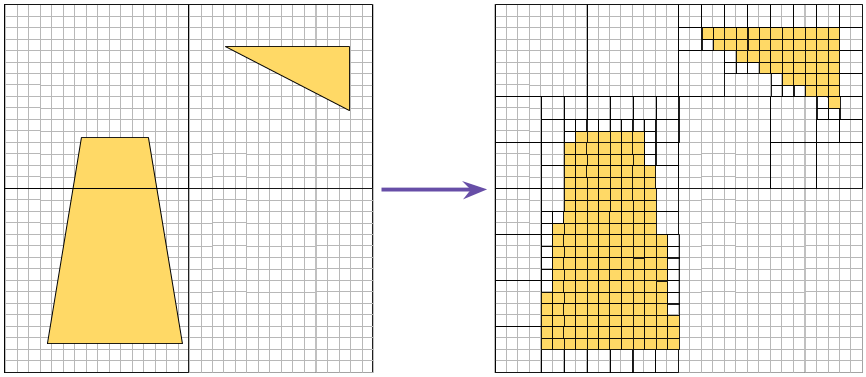
\includegraphics[width=10cm]{grid_decomposition.png}
	\centering
	\caption{A Grid Decomposition scenario.}
	\label{fig:grid_decomposition}
\end{figure}

\subsection{Visibility Graph}
This is another approach belonging to the offline path planning algorithm family. In particular, this approach aims at discovering the shortest obstacle-free path by applying a shortest path algorithm (\emph{e.g.} Dijkstra) on a graph representing a map of obstacle positions and distances in the environment, called the \emph{Visibility Graph}.
Such graph is created as follows:
\begin{itemize}
	\item \textbf{nodes:} vertex points of every obstacle in the environment, in addition to start and destination points;
	\item \textbf{edges:} segments between each pair of nodes that does not intersect an obstacle;
	\item \textbf{weights:} euclidean distances between vertices in the environment;
\end{itemize}

The implementation of the method for this project is slightly different from its original definition due to the assumption of a grid-partitioned environment. Therefore, the following adjustments have been applied:
\begin{itemize}
	\item each node of the Visibility Graph is a cell of the grid
	\item the considered nodes are the the start cell, the destination cell and each obstacle vertex cell
	\item obstacle vertex cells are detected by checking the surrounding configuration of the environment of each obstacle cell as described in Fig. \ref{fig:obstaclevertex};
	\item edges are obtained by creating \emph{dummy paths} between each possible pair of node cells; a dummy path is defined as the simplest path between two cells, ignoring obstacles; only dummy paths without obstacles are considered edges for the Visibility Graph;
	\item the weight for each edge is the number of cell its dummy path is composed of.
\end{itemize}

The shortest path algorithm is then executed on the graph obtained as described above, in order to find the best available path from the start node to the destination node.

\begin{figure}[]
	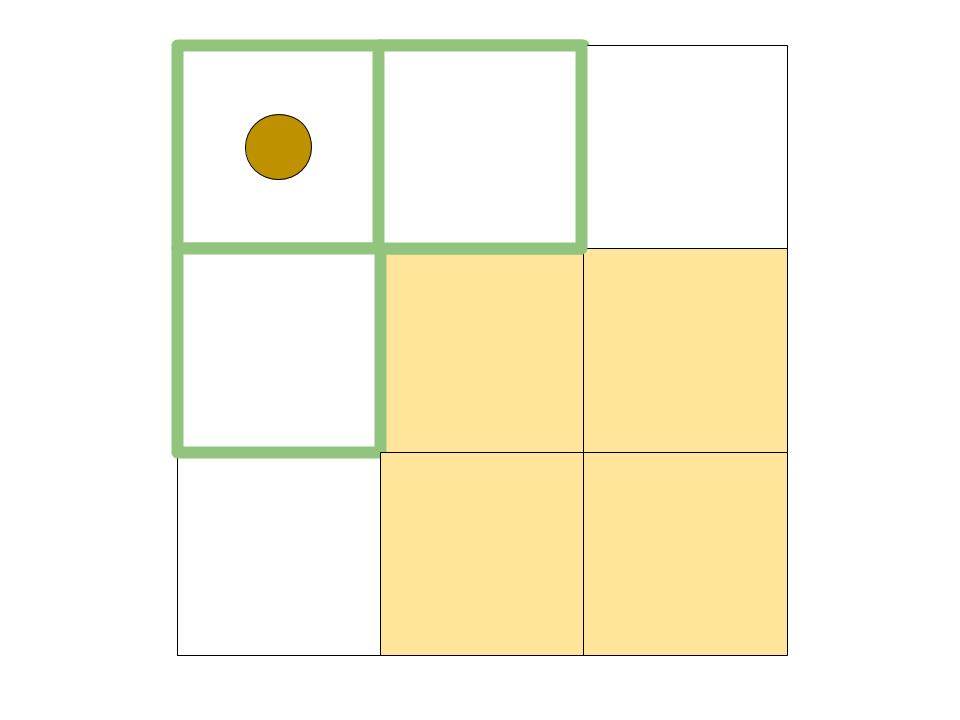
\includegraphics[width=6cm]{obstaclevertex.jpg}
	\centering
	\caption{Example of obstacle vertex detection method. The considered obstacle is the one in the central cell. Adjacent cells in N, W and NW directions are empty. Therefore diagonal cell NW is considered as an obstacle vertex. Of course the algorithms has to check also the other three diagonals.}
	\label{fig:obstaclevertex}
\end{figure}

\begin{figure}[]
	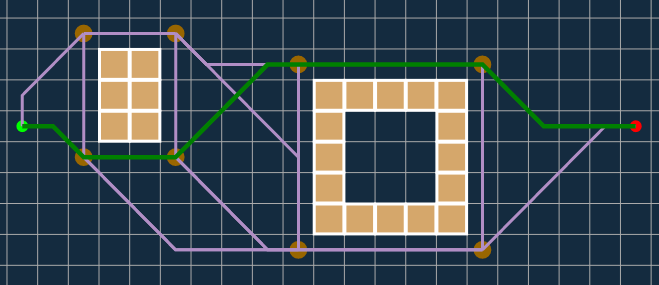
\includegraphics[width=6cm]{visibilityexample.png}
	\centering
	\caption{Example of a visibility graph and the best path.}
	\label{fig:visibilityexample}
\end{figure}

\subsection{Probabilistic Roadmap}
This method follows the same general principles of the Visibility Graph. It represents the environment as a graph and then apply a shortest path algorithm. The main difference is in the procedure that builds the graph, which is highly simplified. The nodes of the graph are a set of randomly selected free cells in the grid, plus the start and the destination cells. The cardinality of the nodes set is the number of cells in the x axis of the map grid. Edges and weight are obtained in the same way as in the Visibility Graph.

\subsection{Potential Fields}
The main idea on which this method is based is to replicate the natural potential field, like the ones generated by gravity or charged particles. The agent should be attracted by the goal and repelled by obstacles: the combination of attractive and repulsive forces will move the agent in the space. The classic definition of this method has been modified to allow its usage in a grid-based discrete environment.

For each empty cell of the grid, the attractive potential field is calculated with the formula:
\[ Attr_{x,y} = (x - x_{goal})^2 + (y - y_{goal})^2 \]
Therefore, the destination corresponds to the global minimum, having his attractive potential field set to zero. On the other hand, every obstacle cell has a potential value set to infinity.

The repulsive field is characterized by two parameters: the distance of influence and the repulsive value. Each obstacle cell create a repulsive force to each empty cell (except for the goal cell) within its distance of influence. The magnitude of this force is given by the repulsive value divided by the distance.
\[Rep_{x,y} = \frac{RepulsiveValue}{\sqrt{(x - x_{ClosestObst})^2 + (y - y_{ClosestObst})^2}}\]
The potential field is the sum, for each cell, of the attractive and repulsive fields.
\[ Pot_{x,y} = Attr_{x,y} + Rep_{x,y} \]
To compute the path to the goal the agent iteratively selects, at each step, the adjacent cell with the lowest potential field value. In this project this method has been referred to as \emph{Simple Potential Fields}.

As described, such approach is too simplistic. In fact, the agent ends up in local minimums too often, even with simple configurations of obstacles (see Fig. \ref{fig:potentialfield}). In order to mitigate these situations, an improved version of the algorithm has been implemented, a variant called \emph{Potential Fields with Memory}, where the agent is able to remember the path that it took to get to its current position. At each step the agent is forced to move to the adjacent cell that has the lowest value between the ones not already in its path.

\begin{figure}[]
	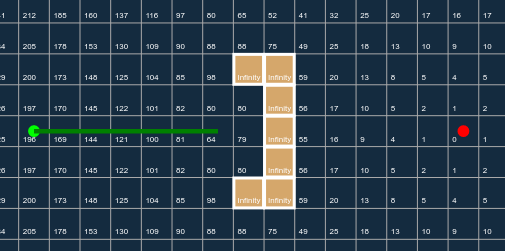
\includegraphics[width=7cm]{potentialfield.png}
	\centering
	\caption{Example of a Potential Fields algorithm stuck into a local minimum.}
	\label{fig:potentialfield}
\end{figure}

\begin{figure}[]
	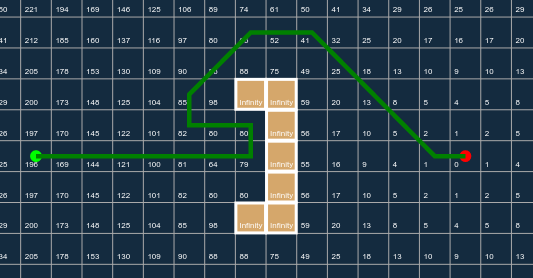
\includegraphics[width=7cm]{potentialfieldmemory.png}
	\centering
	\caption{Potential Fields with Memory can reach the destination in a scenario where Simple Potential Fields would fail
		(see Fig. \ref{fig:potentialfield}).}
	\label{fig:potentialfieldmemory}
\end{figure}

\subsection{Bug Algorithms}
Unlike other path planning algorithms, a Bug approach only assumes to have a local knowledge of the environment, plus destination it must reach. Therefore, it is not possible to establish an \emph{a priori} path, but instead the path will be defined in real time, \emph{i.e.} \emph{online}. Since the family of Bug algorithms is vast, for the purpose of this work the three most common approaches have been taken into account: Bug v1, Bug v2 and Tangent Bug.
Given that at a certain point all the three algorithms assume that the agent follows the perimeter around the obstacle, a key function of the algorithms resulted to be the one that describes how the agent can achieve such behavior, independently from the shape of the obstacle. Such function, called \emph{circumnavigate()} for further reference, is a recursive function whose core behavior is common for all the three algorithms, while the termination conditions changes depending on the case.

\begin{figure}[]
	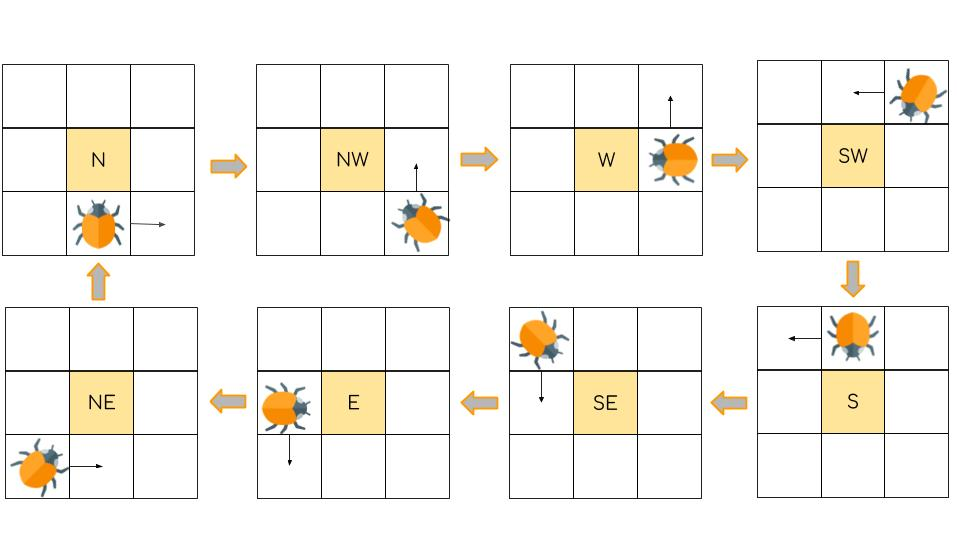
\includegraphics[width=8cm]{circumnavigate.jpg}
	\centering
	\caption{Agent behavior when meeting an obstacle: depending on his current position and the position of the obstacle, the function defines the steps to cover in order to move along the obstacle perimeter. Note that the following figure shows a clockwise movement, but the procedure can be adapted to move in the opposite way without effort. }
	\label{fig:circumnavigate}
\end{figure}

As shown in Fig. \ref{fig:circumnavigate}, the function \emph{circumnavigate()} computes the next step based on the direction in which the obstacle is placed with respect to the bug position.
The figure represents the simplest case, in which the obstacle consists of a single cell; in case of more complex scenarios the function will be called recursively, following the path along the obstacle perimeter, as represented in Fig. \ref{fig:bigObs}.
\begin{figure}[]
	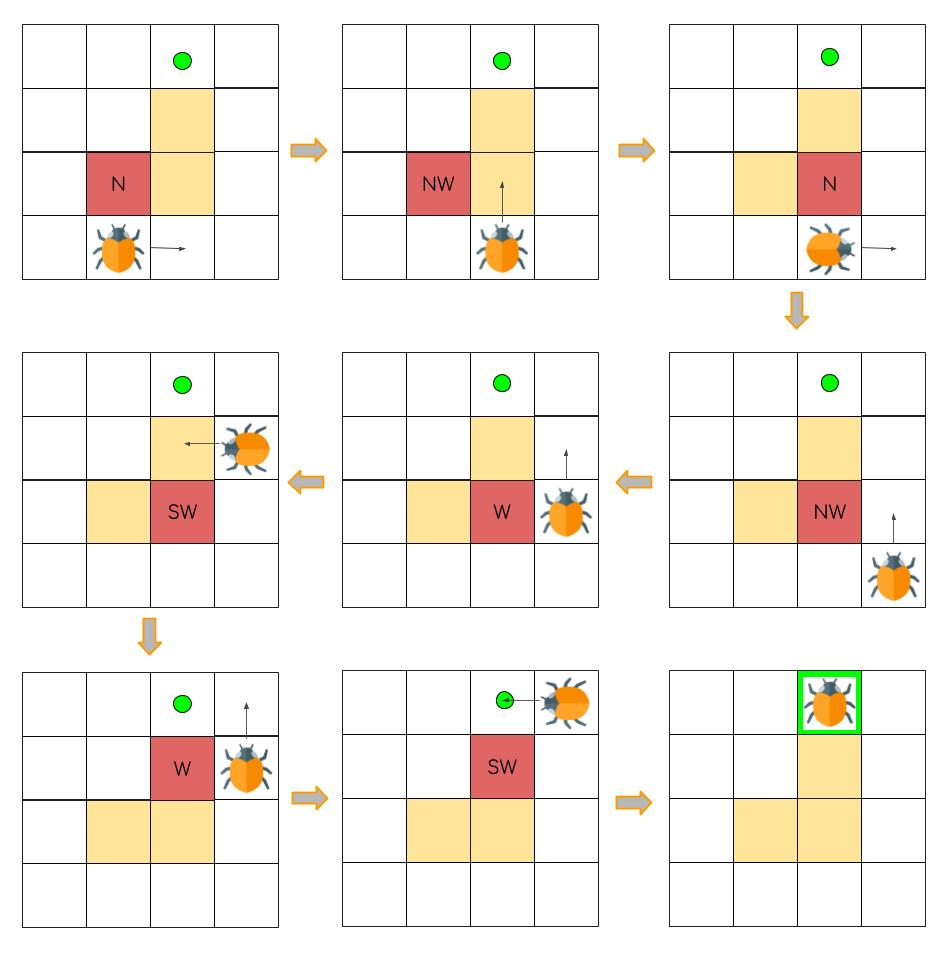
\includegraphics[width=8cm]{bigObs.jpg}
	\centering
	\caption{Bug behavior when meeting a complex obstacle. The red cell indicates the obstacle cell considered at the current time step.}
	\label{fig:bigObs}
\end{figure}

The three considered approaches are now described in details.

\subsubsection{Bug v1}
The algorithms can be summarized as follows:
\begin{itemize}
	\item move by following the simplest path toward the goal (\emph{i.e.} the \emph{dummy path} in the code);
	\item if an obstacle is encountered, move around it computing at each step the distance to the goal;
	\item when the obstacle perimeter has been completely explored, return the to nearest point to the goal around the obstacle;
	\item repeat from step 1 until the goal is reached.
\end{itemize}

As described above, the termination conditions of the \emph{circumnavigate} function (\emph{circumnavigate1} in the code) are the following:
\begin{itemize}
	\item the next step corresponds to the goal;
	\item the next step corresponds to the first that was already covered along the circumnavigation path;
\end{itemize}

The recursive calls are two, addressing the two remaining cases:
\begin{itemize}
	\item the next step corresponds to a free cell, therefore the next call of the function will consider as current position of the bug the new step (because he can move) and as obstacle the same of the current recursion step;
	\item the next step corresponds to an obstacle cell, therefore the next call of the function will consider as current position the last one (because he cannot actually move), and as obstacle the just found next step (because it is a wall).
\end{itemize}

Algorithm \ref{code:circumnavigate1} shows the pseudo-code of \emph{circumnavigate1}.

\begin{algorithm}
	compute newStep along the obstacle\;
	compute the distance to the goal\;
	add the newStep and the distance to the result\;
	\eIf{newStep is the goal or the circumnavigation is complete}{
		\Return res\;
	}{
		\eIf{newStep is not an obstacle}{
			\Return circumnavigate1(newStep, obstacle, end, res)\;
		}{
			remove the last res entry\;
		}
	}
	\Return circumnavigate1(lastStep, newStep, end, res)\;
	\label{code:circumnavigate1}
	\caption{Circumnavigate1(lastStep, obstacle, end, res)}
\end{algorithm}

Since an agent can encounter more obstacles along the way, \emph{circumnavigate1} is called at every encounter, and when it returns the \textit{dummy path} from the point in which the bug stops to follow the obstacle to the destination is computed and followed until a new obstacle or the destination itself is reached.

\subsubsection{Bug v2}

This algorithm is very similar to the previous one, but it has some improvement in the length of the goal path. It can be summarized as follows:
\begin{itemize}
	\item step forward, following the simplest path toward the goal (\emph{dummy path};
	\item if an obstacle is encountered, move along its perimeter until the \emph{dummy path} is reached again;
	\item repeat from the first step until the goal is reached.
\end{itemize}

This means that the termination conditions of the \emph{circumnavigate} function (\emph{circumnavigate2} in the code) in this case are following:
\begin{itemize}
	\item the next step corresponds the goal;
	\item the next step is included in the dummy path;
\end{itemize}

While the recursive calls are the same of Bug v1.

Algorithm \ref{code:circumnavigate2} shows the pseudo-code of \emph{circumnavigate2}, which is easier than the previous one. In the pseudo-code, \emph{oldPath} represents the \emph{dummyPath}.

\begin{algorithm}
	compute newStep along the obstacle\;
	add the newStep to the newPath //\emph{ newPath is the path around the obstacle}\;
	\eIf{newStep is in oldPath}{
		\Return newPath\;
	}{
		\eIf{newStep is not an obstacle}{
			\Return circumnavigate2(newStep, obstacle, newPath, oldPath)\;
		}{
			remove the last entry from newPath\;
		}
	}
	\Return circumnavigate1(lastStep, newStep, newPath, oldPath)\;
	\label{code:circumnavigate2}
	\caption{Circumnavigate1(lastStep, obstacle, newPath, oldPath)}
\end{algorithm}

Similarly to v1, Bug v2 may call \emph{circumnavigate2} many times, as there can be many obstacles along the path. Unlike v1, it is now easier to restart moving over the \emph{dummyPath}, since the path will not mutate after the circumnavigation.

\subsubsection{Tangent Bug}
This is the most complex approach among this family of algorithms. What really distinguishes it from the others is the assumption that the bug is capable of sensing the area around it within a given range. Starting from the assumption that the environment is defined by a grid, the sensed area will be defined by a square around the bug as represented in Fig. \ref{fig:range}. In the image it is possible to notice that all the cells within the sensing range have a distance from the bug $<= r$ (2 in this case).

The behavior of this algorithm can be summarized as follows:
\begin{itemize}
	\item follow the \emph{dummy path} until an obstacle is sensed;
	\item detect the point(s) of discontinuity;
	\item compute the heuristic distance to the goal for each discontinuity;
	\item move to the discontinuity point identified by the minimum heuristic distance;
	\item when the discontinuity is reached, move along the obstacle boundary;
	\item while following the obstacle perimeter, compute the shortest distance from the points in the range of the agent to the destination (\emph{dReach}), and also the shortest distance from the points on the perimeter to the destination (\emph{dFollow});
	\item when \emph{dReach} becomes lower than \emph{dFollow}, compute the new \emph{dummy path} to the destination and start over.
\end{itemize}

The heuristic distance is computed as the sum between the distances from the bug to the discontinuity points and from the discontinuity points to the destination.

\begin{figure}[]
	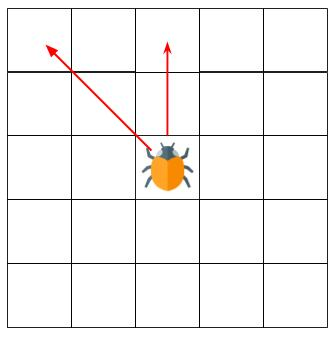
\includegraphics[width=4cm]{rangeArea.jpg}
	\centering
	\caption{The range area sensed by the agent, with r = 2.}
	\label{fig:range}
\end{figure}

Since the grid assumption for our environment causes a non optimal behavior, the procedure has been slightly modified, making \emph{dReach} being computed as the distance between the last step and the destination and \emph{dFollow} as the distance between the last considered obstacle cell and the destination. The perimeter is followed until \emph{dReach} $<$ \emph{dFollow} and there are no obstacles along the \emph{dummyPath} from the actual position to the goal is free for at least one step.
Algorithms \ref{code:tangentBug} and \ref{code:boundaryFollow} show the pseudo-code of tangent bug. The function \emph{boundaryFollow} is equivalent to the \emph{circumnavigate}, but adapted for this approach.

\begin{algorithm}
	pathToDest = []\;
	\While{not reached dst}{
		compute range area\;
		compute discontinuities\;
		\eIf{discontinuities are blocking the dummyPath}{
			find the discontinuity at minimum heuristic distance\;
			go straight to that discontinuity\;
			compute the best direction to follow the obstacle\;
			boundaryFollow(lastStepBeforDiscontinuity, minDiscontinuity, direction, pathToDest)\;
			dummyPath = findDummyPath(lastStep, dest) //last step is the last step along the boundary\;
		}{
			pathToDest.push(currentStep)\;
		}
	}
	\Return pathToDest
	\label{code:tangentBug}
	\caption{tangentBug(dummyPath)}
\end{algorithm}

\begin{algorithm}
	compute newStep along the perimeter obstacle\;
	\eIf{newStep is not an obstacle}{
		path.push(newStep)\;
		\If{newStep = destination}{
			\Return path\;
		}
		dummy = findDummyPath(newStep, destination)\;
		range = rageArea(newStep, 1) // 1 is r\;
		dFollow = pathCost(obstacle,destination)\;
		dReach =  pathCost(newStep, destination)\;
		\If{ not obstacleInPath(dummy, range) AND dReach < dFollow}{
			\Return path
		}
		\Return boundaryFollow(newStep, obstacle, destination, dir, path)\;
	}{
		\Return boundaryFollow(lastStep, newStep, destination, dire, path)\;
	}
	\label{code:boundaryFollow}
	\caption{boundaryFollow(lastStep, obstacle, destination, dir, path)}
\end{algorithm}

\section{Performance evaluation}

\subsection{Offline Algorithms}
The \textit{Decomposition} methods, as implemented in this work, are obviously complete, since they are always able to find the best path to reach the destination if there is one.

The \textit{Visibility Graph} method is also complete. The downside of this approach is its elevated computational cost. In fact, it is necessary to scan every obstacle cell in order to discover the obstacle vertex points, then build the \emph{dummy path} between each pair of vertices and finally apply a shortest path algorithm.

The \textit{Probabilistic Roadmap} approach tries to mitigate this problem by randomly selecting nodes of the graph. However, it still has to create all the \emph{dummy paths} that are used as the edges of the graph. Obviously, the path obtained using this algorithm is not guaranteed to be the best possible; in fact, it may even not find a path even if there is one.

There is a tradeoff between the time needed to compute and the number of random samples in the map: increasing the number of nodes increases the chance to find a shortest path, but requires more computational time to create the edges.

\textit{Simple Potential Fields} has proven to be too weak to be used without any adjustment. The agent gets stuck in local minimums even in scenarios with just a few obstacles.

The reason above is exactly why \textit{Potential Fields with Memory} has been implemented. It is just a simple addition to the Potential Fields approach, but shows significant improvements.
Strong and weak scenarios can also heavily depend on repulsive values and distance of influence of obstacles.

\subsection{Online Algorithms}
\textit{Bug v1}, despite using a naive approach and therefore being non optimal, is complete; compared to Bug v2, the latter is able to find shorter paths, as shown in Fig. \ref{fig:Bug1vsBug2}.
Nevertheless, this performance improvement has a cost, since in some configuration Bug v2 can get stuck in loop while searching for path to the destination; an example is shown in Fig. \ref{fig:spiral}.

\begin{figure}[]
	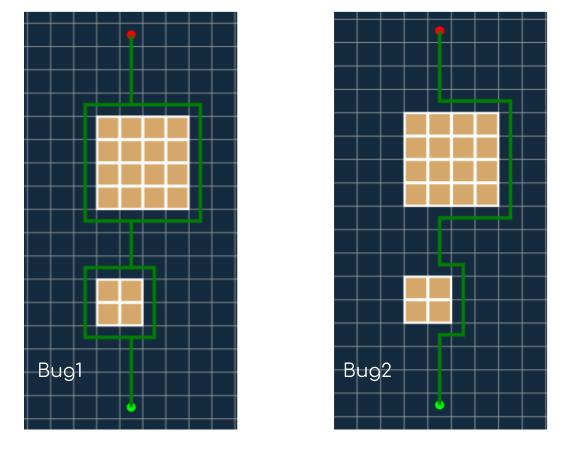
\includegraphics[width=8cm]{Bug1vsBug2.jpg}
	\centering
	\caption{Bug v1 and Bug v2, compared in the same environment.}
	\label{fig:Bug1vsBug2}
\end{figure}

\begin{figure}[]
	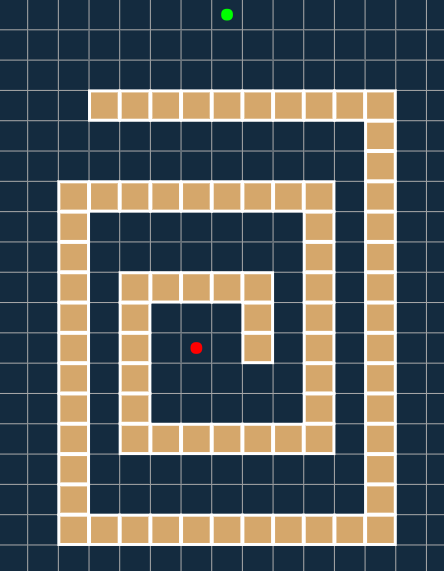
\includegraphics[width=6cm]{spiral.png}
	\centering
	\caption{An example of configuration in which Bug v1 can find a path, while Bug v2 can't.}
	\label{fig:spiral}
\end{figure}

The implementation of Tangent Bug can find even shorter paths compared to Bug v2 (as shown in Fig. \ref{fig:tgbug}), but similarly it can sometimes get stuck in loops. Also, it can happen that the goal path found by Tangent Bug results longer than the one found by Bug v2, as shown in Fig. \ref{fig:bug2vstgbug}.

\begin{figure}[]
	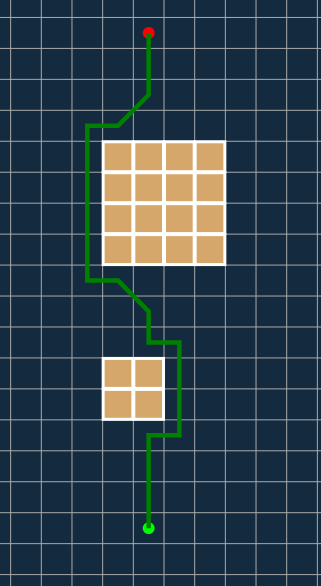
\includegraphics[width=4cm]{tgbug.png}
	\centering
	\caption{Tangent Bug, applied in the same configuration shown in Fig. \ref{fig:Bug1vsBug2}, results in a shorter path.}
	\label{fig:tgbug}
\end{figure}

\begin{figure}[]
	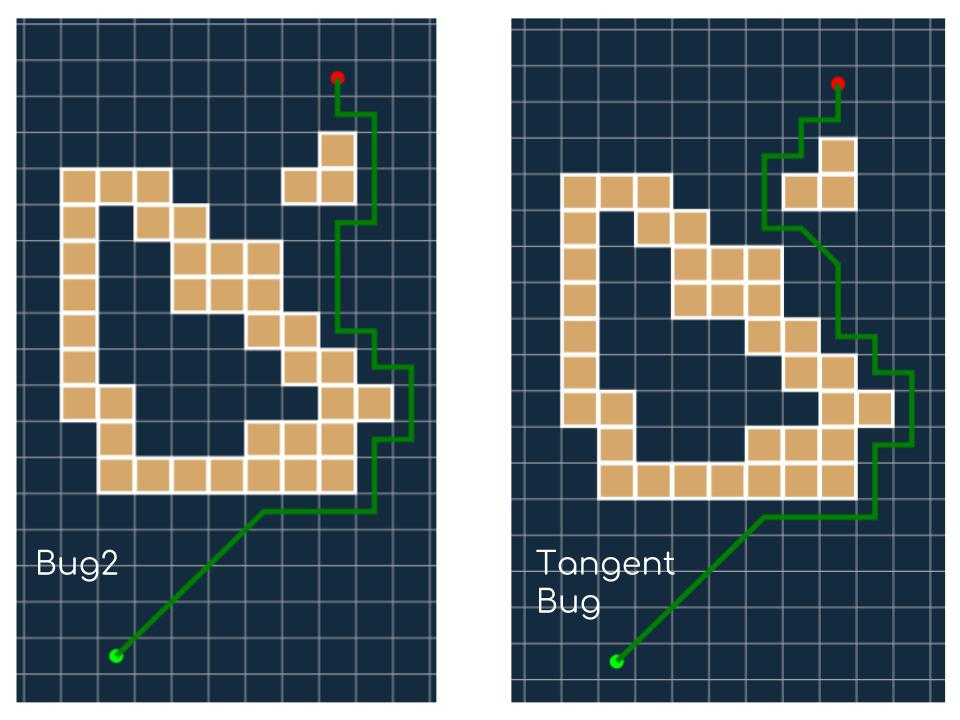
\includegraphics[width=8cm]{bug2vstgbug.jpg}
	\centering
	\caption{Bug v2 and Tangent Bug in the same configuration.}
	\label{fig:bug2vstgbug}
\end{figure}

\section{Conclusions}
In this report we described our implementation and analysis of the most popular path planning algorithms and approaches.

The output of our work resulted to be \textbf{Path Planner} \cite{Path-Planner}, a JavaScript application which allows to experiment and tests the different approaches in a practical way over bi-dimensional grid-based environment.

On the other hand, our work allowed us to gain knowledge and to better understand and test different path planning approaches. Both the software produced and this knowledge will be used to accomplish the second part of our project, which aims at implementing a path planning methodology in a rover equipped with sensors, moving in a real-world environment with obstacles.

\bibliographystyle{unsrt}
\bibliography{report}
\end{document}